\section{Qualitative Evaluation}

\subsection{Visual Comparison Across Models}

% AGE vs SAGE vs SFSAGE
% Same input, same dataset
% Highlight realism, diversity, edit strength

\begin{figure}[H]
\centering
\setlength{\tabcolsep}{2pt}

\begin{tabular}{ccccccc}
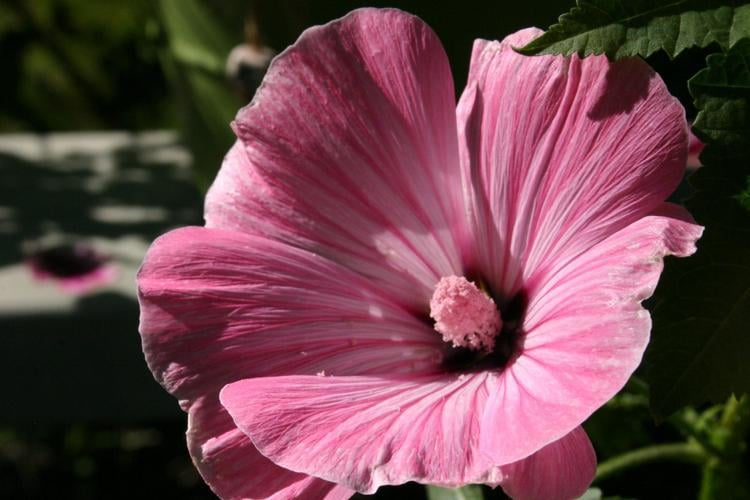
\includegraphics[width=0.14\textwidth,height=0.14\textwidth]{images/input_1.jpg} &
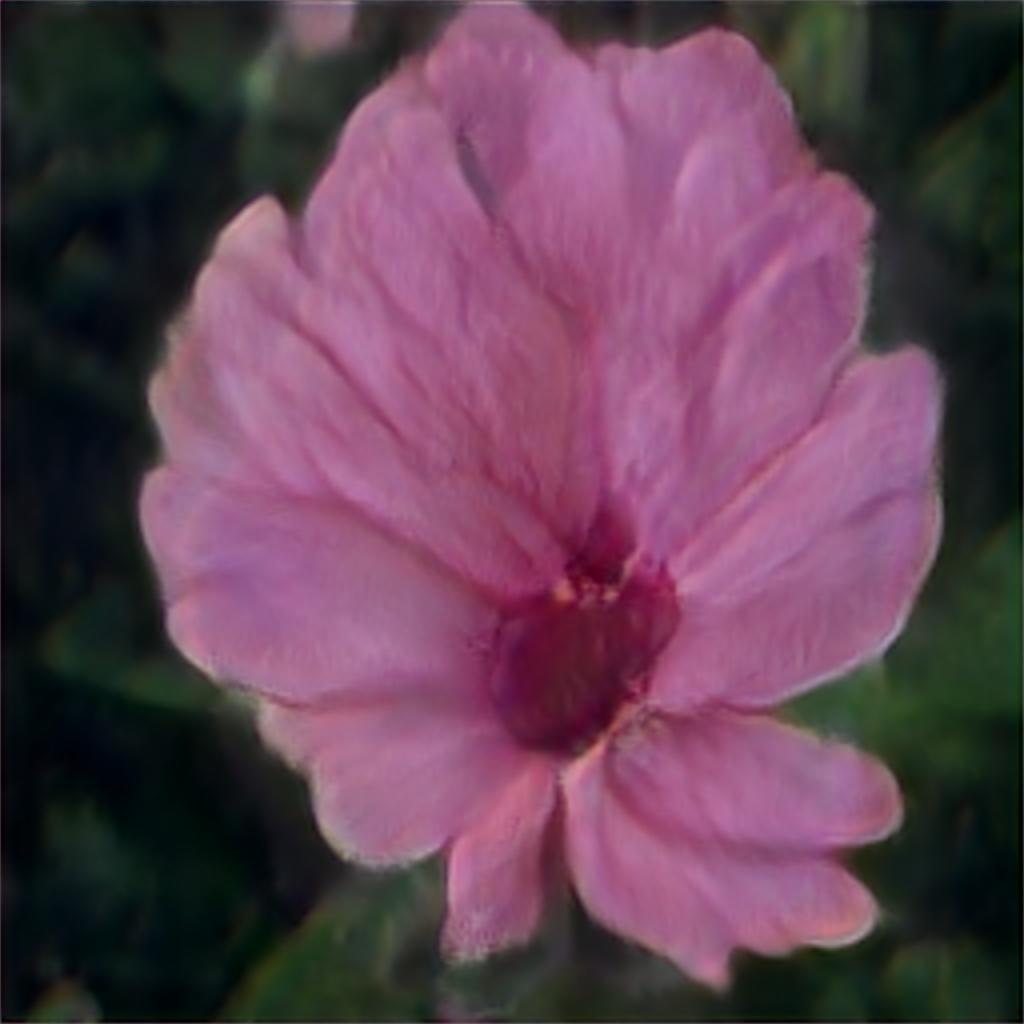
\includegraphics[width=0.14\textwidth,height=0.14\textwidth]{images/1age_output1.jpg} &
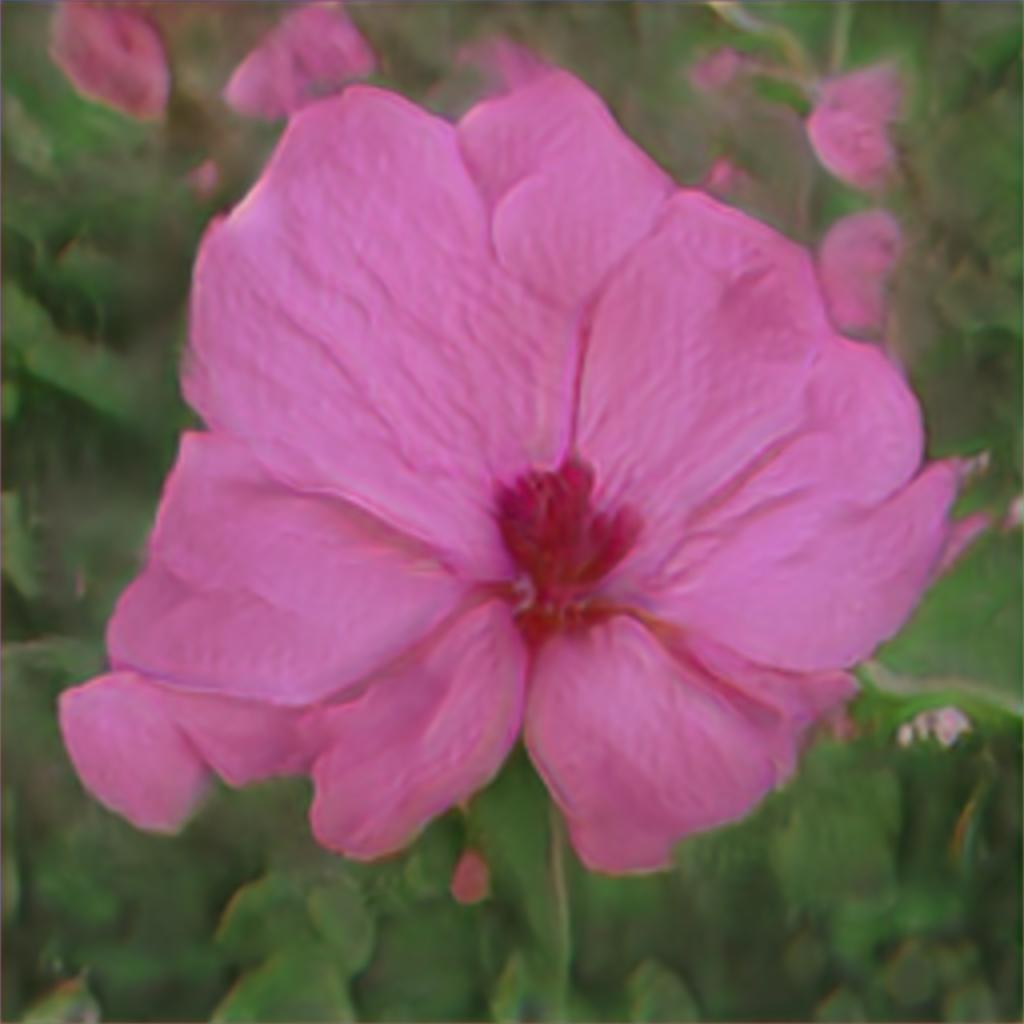
\includegraphics[width=0.14\textwidth,height=0.14\textwidth]{images/1age_output2.jpg} &
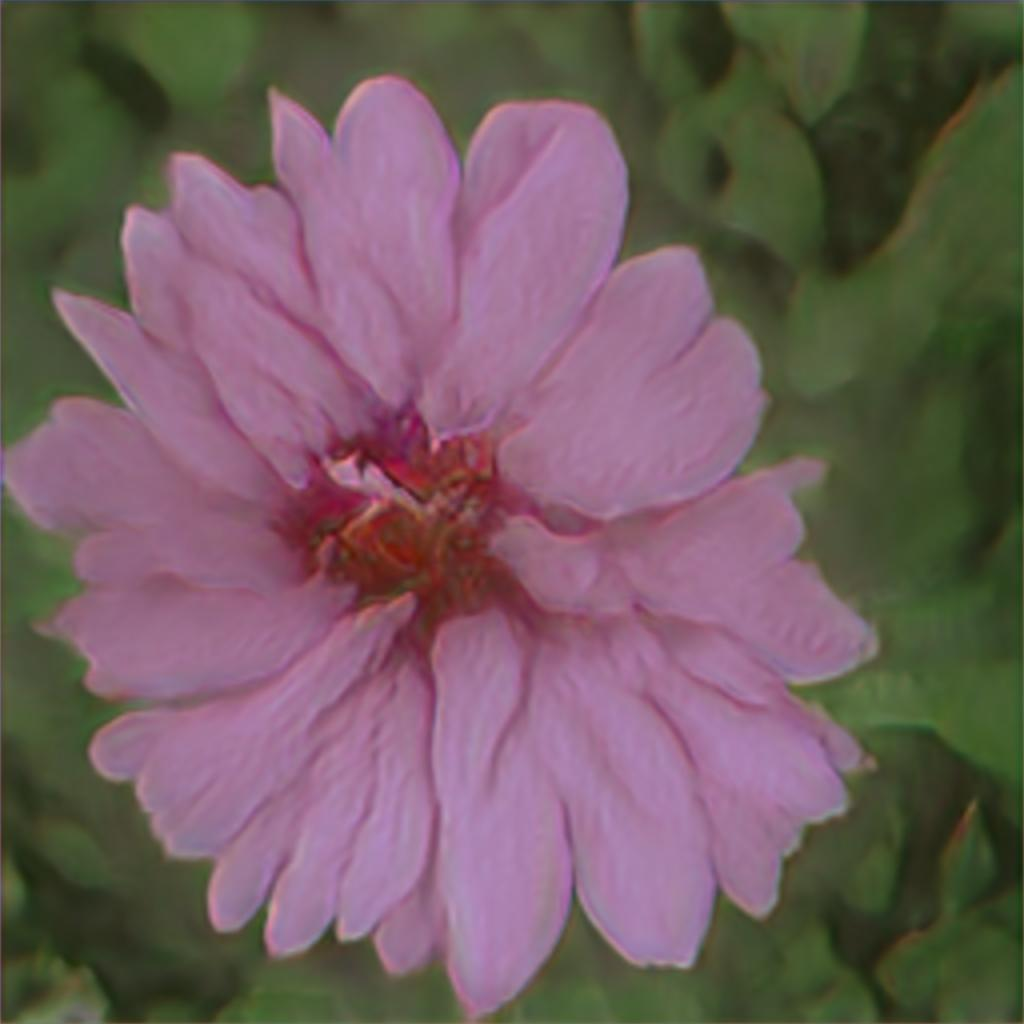
\includegraphics[width=0.14\textwidth,height=0.14\textwidth]{images/1sage_output1.jpg} &
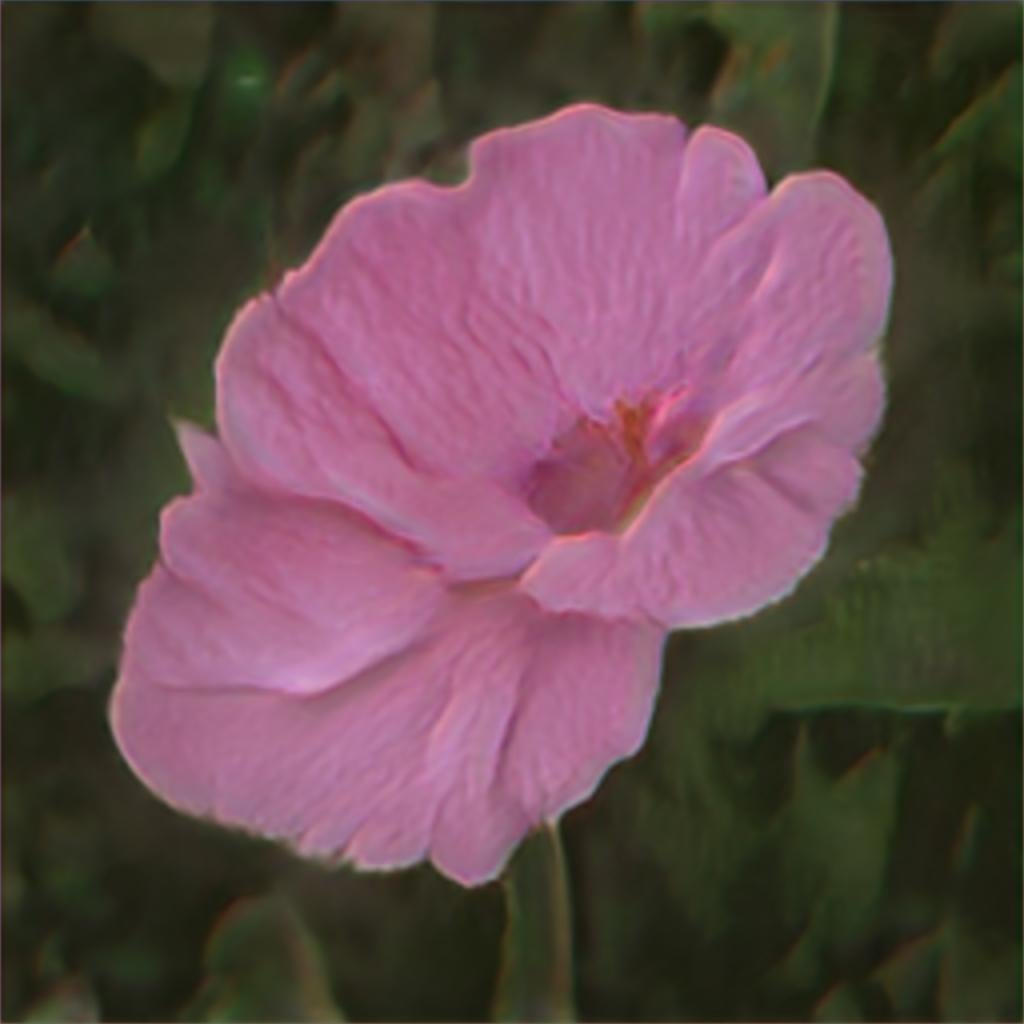
\includegraphics[width=0.14\textwidth,height=0.14\textwidth]{images/1sage_output2.jpg} &
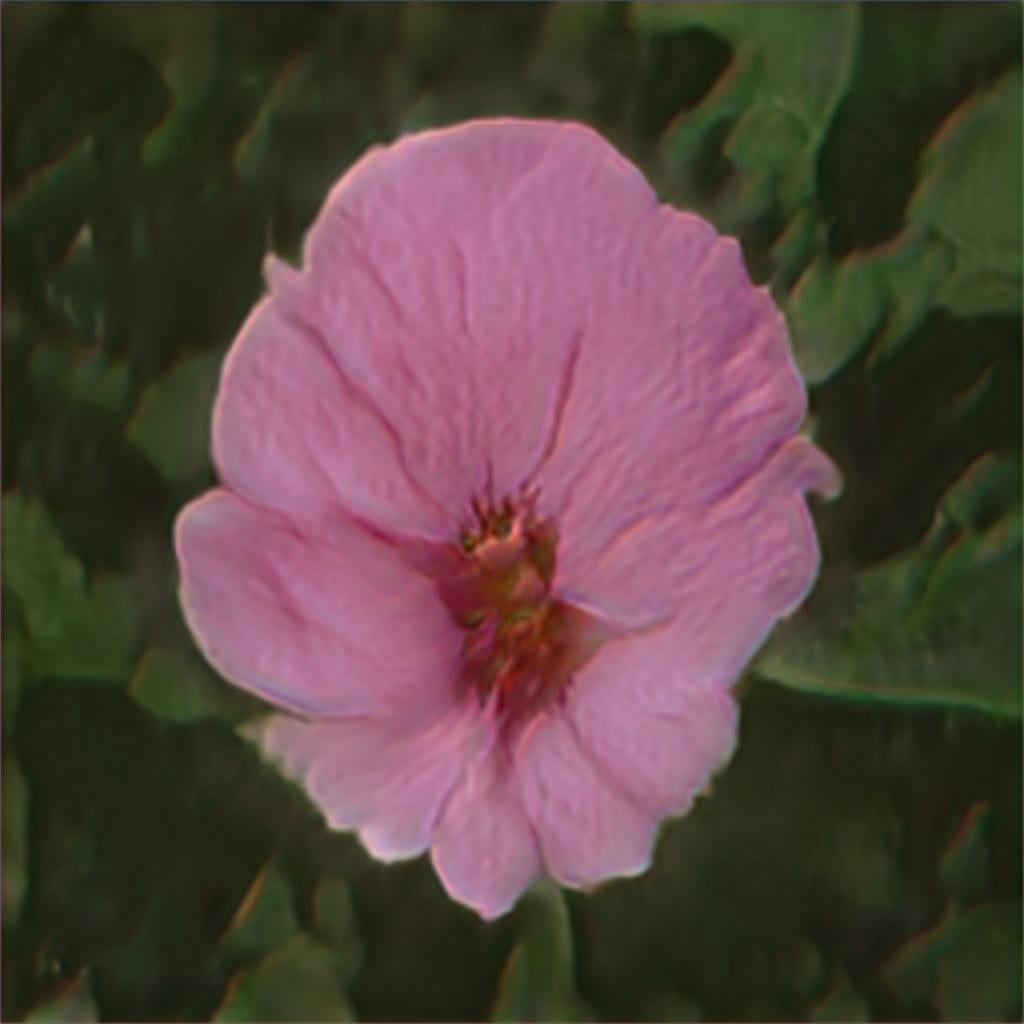
\includegraphics[width=0.14\textwidth,height=0.14\textwidth]{images/1sfsage_output1.jpg} &
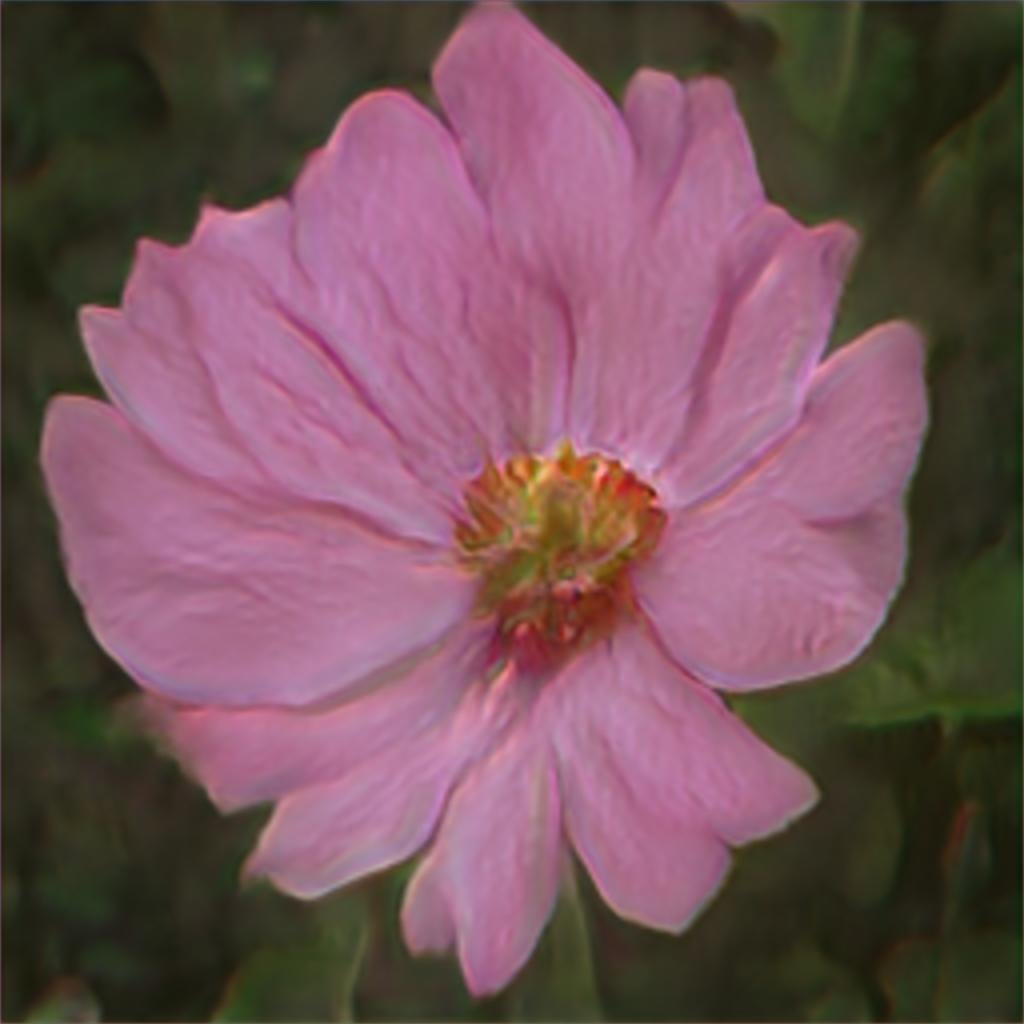
\includegraphics[width=0.14\textwidth,height=0.14\textwidth]{images/1sfsage_output2.jpg}
\\
Input & AGE & AGE & SAGE & SAGE & SFSAGE & SFSAGE
\end{tabular}

\caption{Comparison across AGE, SAGE, and the proposed SFSAGE model under one-shot setting, where a single reference image is used to condition the model during inference.}
\label{fig:qualitative_comparison}
\end{figure}


\begin{figure}[H]
\centering
\setlength{\tabcolsep}{2pt}

\begin{tabular}{ccccccc}
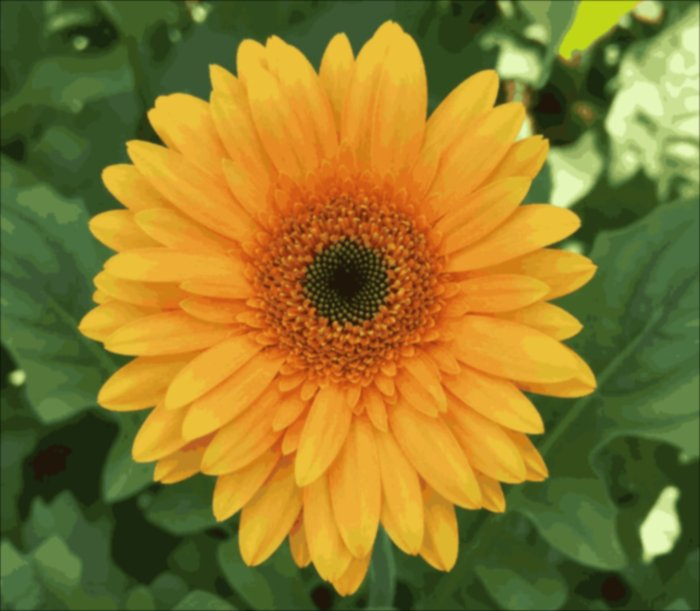
\includegraphics[width=0.14\textwidth,height=0.14\textwidth]{images/input_2.png} &
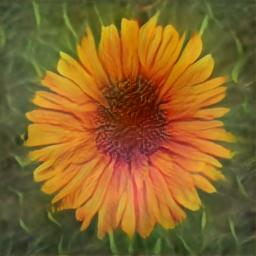
\includegraphics[width=0.14\textwidth,height=0.14\textwidth]{images/2age_output1.jpg} &
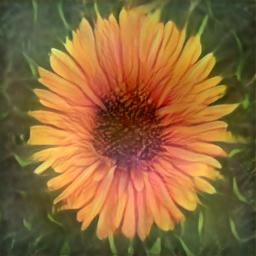
\includegraphics[width=0.14\textwidth,height=0.14\textwidth]{images/2age_output2.jpg} &
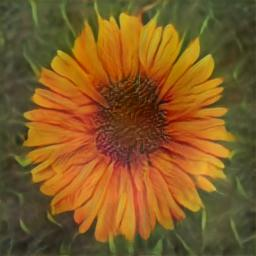
\includegraphics[width=0.14\textwidth,height=0.14\textwidth]{images/2sage_output1.jpg} &
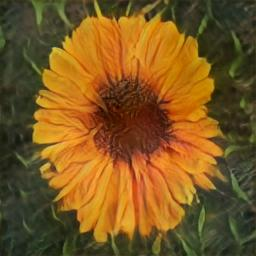
\includegraphics[width=0.14\textwidth,height=0.14\textwidth]{images/2sage_output2.jpg} &
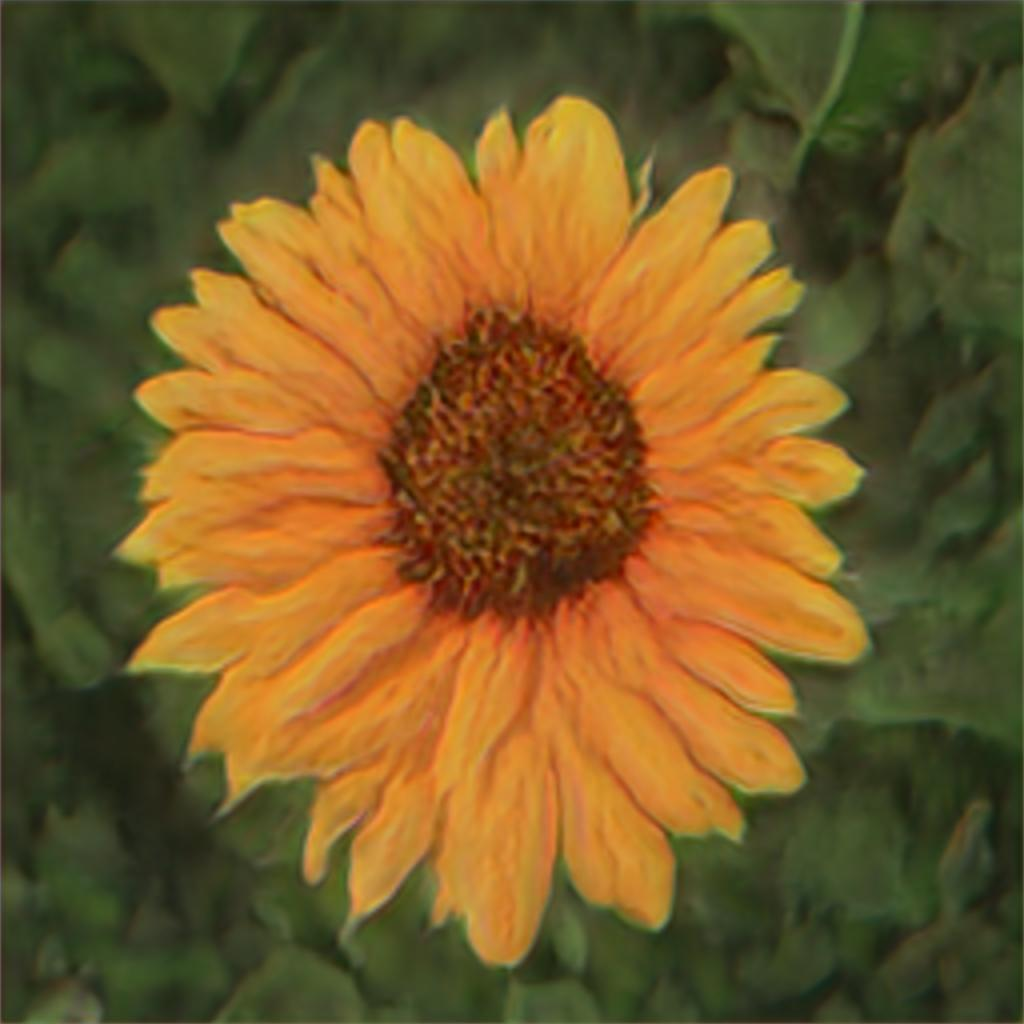
\includegraphics[width=0.14\textwidth,height=0.14\textwidth]{images/2sfsage_output1.jpg} &
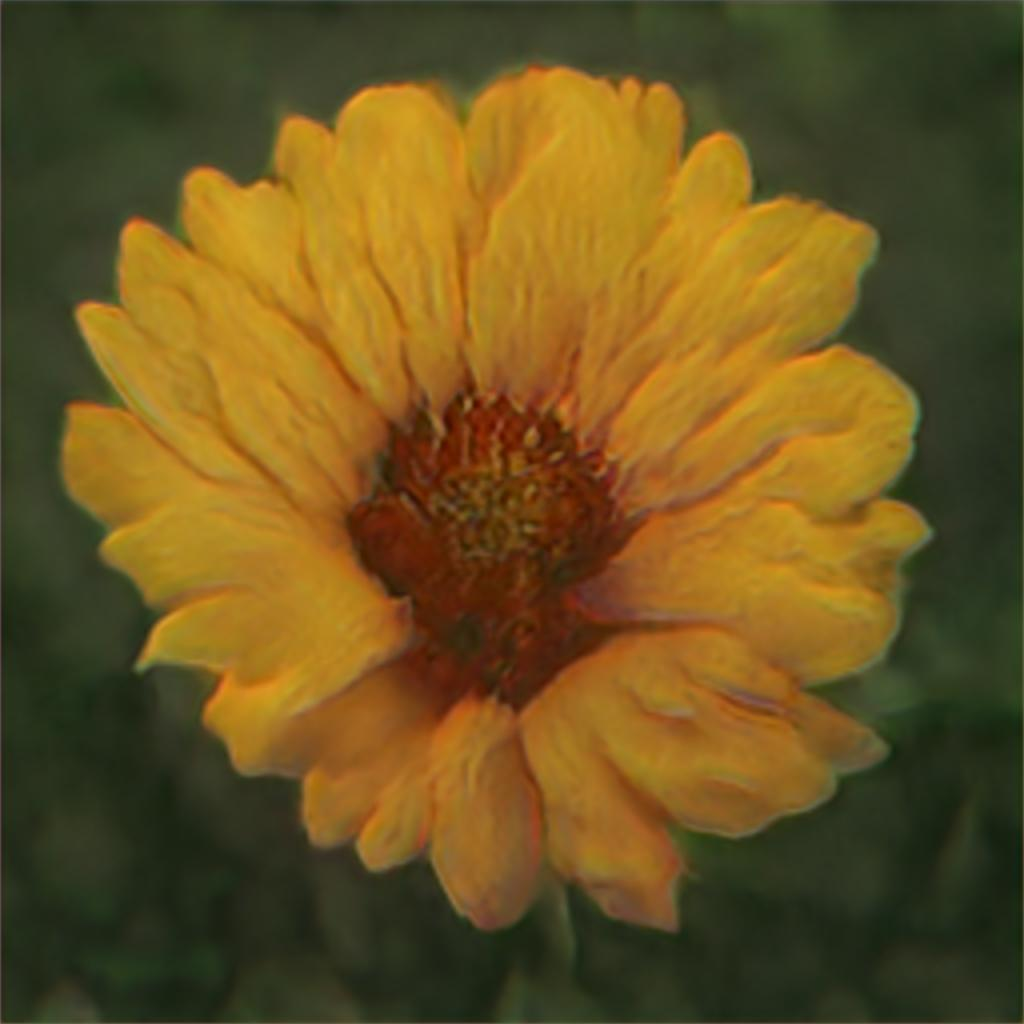
\includegraphics[width=0.14\textwidth,height=0.14\textwidth]{images/2sfsage_ouptut2.jpg}
\\
Input & AGE & AGE & SAGE & SAGE & SFSAGE & SFSAGE
\end{tabular}

\caption{Comparison across AGE, SAGE, and the proposed SFSAGE model under one-shot setting with a different image input.}
\label{fig:qualitative_input2}
\end{figure}

% image names for af:
% input3.png, age_af_output1.jpg, age_af_output2.jpg, sage_af_output1.jpg, sfsage_af_output1.jpg, sage_output2.jpg, sfsage_af_ouptut2.jpg

\begin{figure}[H]
\centering
\setlength{\tabcolsep}{2pt}

\begin{tabular}{ccccccc}

\includegraphics[width=0.14\textwidth,height=0.14\textwidth]{images/input3.jpg} &
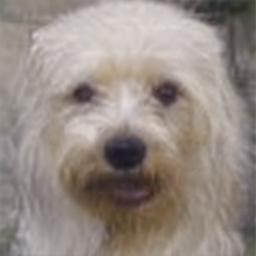
\includegraphics[width=0.14\textwidth,height=0.14\textwidth]{images/age_af_output1.jpg} &
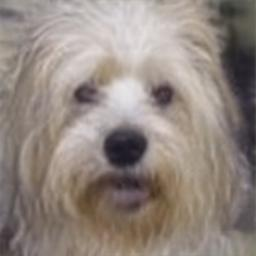
\includegraphics[width=0.14\textwidth,height=0.14\textwidth]{images/age_af_output2.jpg} &
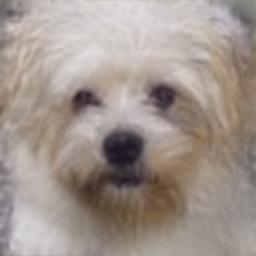
\includegraphics[width=0.14\textwidth,height=0.14\textwidth]{images/sage_af_output1.jpg} &
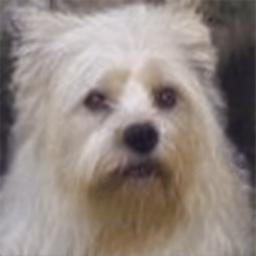
\includegraphics[width=0.14\textwidth,height=0.14\textwidth]{images/sage_output2.jpg} &
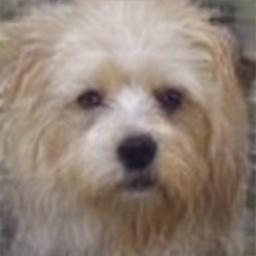
\includegraphics[width=0.14\textwidth,height=0.14\textwidth]{images/sfsage_af_output1.jpg} &
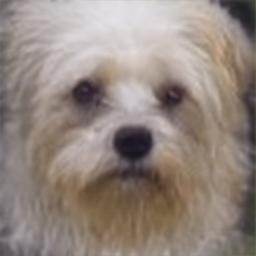
\includegraphics[width=0.14\textwidth,height=0.14\textwidth]{images/sfsage_af_ouptut2.jpg} \\
Input & AGE & AGE & SAGE & SAGE & SFSAGE & SFSAGE
\end{tabular}

\caption{Comparison across AGE, SAGE, and the proposed SFSAGE model on the Animal Faces dataset under one-shot setting. Each model generates two outputs per input image to demonstrate edit diversity and semantic consistency.}
\label{fig:qualitative_animalfaces}
\end{figure}


\subsection{Visual Observations}

\subsubsection{Flowers}

Figures \ref{fig:qualitative_comparison} and \ref{fig:qualitative_input2} describe the qualitative analysis of the results of the edited flowers 
based on the baseline models AGE and SAGE, and the proposed model SFSAGE. The models are compared with regard to their ability to maintain the 
colors properly, the sharpness of the images, the level of contrast, and realism. As shown in Figure \ref{fig:qualitative_comparison}, the proposed 
model performs well in the retention of the pink petal colors from the input images. It also performs much better based on the level of semantic 
consistency. Note that the proposed model also fails to represent the combined red and yellow colors of the pistil from the input images. On the 
other hand, the proposed model performs much better than both the input images in the sharpness of the petal. Although there are inconsistencies 
from the input images, the proposed model also performs much better. In addition, the level of contrast in the proposed model results in the sharpest 
flower among all the models. Further, the advantages of SFSAGE are highlighted by Figure \ref{fig:qualitative_input2}. The sharpness in petal edges 
is better retained by the model compared to AGE and SAGE, which allows for a more photo-realistic and organic rendering. More varied outputs have 
also resulted from SFSAGE; for instance, in one generated image, the flower is presented with a slight tilt, reflecting strong attribute manipulation. 
The model maintains higher clarity, with balanced contrast and natural color distribution, while AGE slightly looks pale with reduced contrast in 
areas, which is somewhat settled by SAGE as it balances the contrast. Overall, the 65 generated flower images produced by SFSAGE are the sharpest, 
most realistic, and visually consistent as compared to the other models being tested.

\subsubsection{Animal Faces}

Figure \ref{fig:qualitative_animalfaces} provides a comparison of the outputs produced by the AGE, SAGE, and proposed SFSAGE model on the 
Animal Faces data set using a picture of a dog as input. As observed, the outputs produced by the models have managed to maintain the color 
and texture of the input data, implying success by these models in maintaining basic characteristics produced by each model. Considering the 
clarity and image properties, all the outputs produced by these models can be considered similar, since there is minimal blurring effect and 
texture preservation on the fur of the input image. Consistency and overall properties, on the other hand, differ significantly, since there 
is more diversity apparent in the outputs produced by the AGE and SAGE models, with a slight difference in orientation between the two outcomes 
produced by each model. The more consistent results produced by the proposed SFSAGE model, on the contrary, demonstrate success towards 
maintaining integrity while providing semantic edits. Also, there are some minor enhancements in the realism of the output, whereby the output 
from SFSAGE shows slightly more coherent shading and blending of the fur patterns. This indicates that although all these models demonstrate 
the ability to sustain basic attributes like color and texture, the SFSAGE model has the best consistency in output.